\documentclass{article}
\usepackage{graphicx} % Required for inserting images
\usepackage[margin=1.0in]{geometry}
\usepackage{amsmath}
\usepackage{float}
\usepackage{hyperref}
\usepackage{listings}

\linespread{1}
\setlength{\parindent}{0pt} % Disable paragraph indentation

\title{CPEN 333 Final Project : Part I Alternative (Multithreaded Game)}
\author{Group G6 : Muntakim Rahman and Tomaz Zlindra}
\date{December 6th, 2024}

\begin{document}

\maketitle

\section{Redesign}
Our main redesign of the program structure was to change the model of Inter-Process Communication (IPC) from message passing to shared-memory.
This task was reduced to \texttt{producer-consumer} problems for each resource, in which the \texttt{producer} must wait for the \texttt{consumer} to yield the resource and vice-versa,
in order for the program to be thread-safe. \\

Having removed the use of the \texttt{Queue}, \texttt{QueueHandler} classes, we aimed to achieve synchronization with \texttt{semaphores} for
the \textit{4} shared resources (i.e. "\texttt{game\_over}", "\texttt{score}", "\texttt{prey}", "\texttt{move}") to indicate when they have been produced. All, except for \texttt{"game\_over"}
are accessed via a \texttt{dict} of \texttt{mutexes}. \\

Please see the comment at the top of the \texttt{part1\_alternative.py} file for a description of the implementation. This file will describe the benefits, disadvantages, and challenges of this.

\section{Benefits}

Since we were able to eliminate the need for \textit{2} classes, this simplified the relationships between classes, as shown in Figure \ref{fig:Part1_Alternative_ClassDiagrams}. \\

\begin{figure}[H]
    \centering
    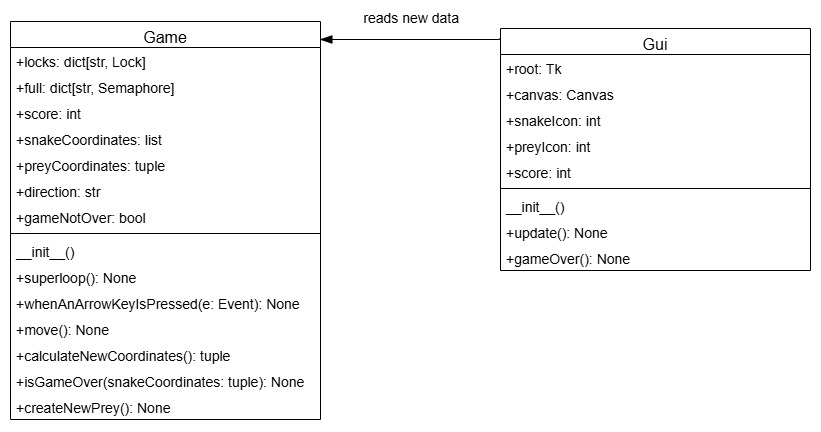
\includegraphics[width=0.9\textwidth]{../Part_1_Alternative_ClassDiagrams.jpg}
    \caption{Part 1 Alternative - UML Relationship}
    \label{fig:Part1_Alternative_ClassDiagrams}
\end{figure}


\section{Disadvantages}

A single producer / consumer is accessing the resource at all times and we need to ensure there isn't a race condition between them. This is a problem we have addressed before (e.g. Lab 5).
We have implemented this rather simply, and aren't treating them as \texttt{reader-writer} for our synchronization problem (i.e. \( \{ \text{Producers, Consumers}\, \} \cup \{ 0, 1 \} \)).

\subsection{Complexity}

That said, there is added complexity from the original design. We now have to ensure that each of the \textit{4} shared resources are accessed effectively. More locks means that there are more critical sections to manage among threads.
This in turn, leads to more potential complexity. We needed to ensure that critical sections were kept short and to the point.
\textit{If we abstract this as a \texttt{reader-writer} problem momentarily : \texttt{readers} access the current data and use it for their needs, \texttt{writers} update the new data.}

Having the \texttt{full} semaphores to indicate when a new value is available adds another layer of complexity. This condition must be evaluated by the \texttt{consumer} once it successfully acquires a lock. \\

\textit{Note that the \texttt{game} instance acts as both a reader and a writer in different places. It reads the current value(s) of the shared resource and copies it for processing.It also writes the new data to the shared resource} \\

\subsection{Overhead}

We also need to store the \texttt{game.preyCoordinates} data field for the \texttt{gui} instance to access for its \texttt{Tkinter} widget, which wasn't necessary with the \texttt{queue} implementation.
Here, we are also updating the coordinates every \textit{100\,\,\text{ms}}. This is unnecessary as it should only be done upon change. The \texttt{Queue.get\_nowait()} method had addressed this issue.

\subsubsection{Future Improvements}

To improve this solution, we should treat this as a \texttt{reader-writer} synchronization problem in which multiple \texttt{readers} can be present at any given time. This will likely improve performance and allow perform Improvements
such that it is near identical to the original implementation with the \texttt{Queue}.

\section{Challenges}

We initially spawned two threads for the \texttt{game.superloop()} and \texttt{gui.update()} methods.
This was highly problematic since the program functioned as intended for initial gameplay. Critical sections seemed to be thread-safe both theoretically and in practice.
However, through extensive testing we observed this consistently caused the program to crash when the snake grew at a score \textasciitilde \textit{25-26}. \\

We realized why the original program design had the \texttt{QueueHandler.queueHandler()} method schedule itself with the \texttt{Tk.after(100)} method.
From referring to the \texttt{Python} documentation, we realized that \texttt{Tkinter} widget updates must be done by the main thread.
\textit{(See The Python Software Foundation. (n.d.). Tkinter - Python interface to TCL/TK. Python Documentation. \href{https://docs.python.org/3/library/tkinter.html\#threading-model}{https://docs.python.org/3/library/tkinter.html\#threading-model})}

\subsection{Solution}

Instead of having the \texttt{gui.update()} method conditionally loop in a spinlock, we wrote it to be a conditional statement which schedules itself with the \texttt{Tk.after(100)} method.
We implemented this with non-blocking acquires as well, such that widget updates wouldn't trap the thread in a spinlock (i.e. while waiting) and block other widget updates from occuring in the meantime.

\end{document}
